\documentclass[10pt,letterpaper,twocolumn]{article}

\usepackage[top=2.1cm,left=2.0cm,right=2.0cm,footskip=2.0cm]{geometry}
\usepackage[utf8]{inputenc}     % for Unicode
\usepackage{cite}               % citation
\usepackage[dvipdfmx]{hyperref} % links
\usepackage{caption}            % caption
\usepackage{microtype}          % improves typesetting in LaTeX
\usepackage{algpseudocode}
\usepackage{algorithm}
\usepackage{graphicx}
\usepackage{color} % ex.) \textcolor{color}{text}

\renewcommand{\algorithmicrequire}{\textbf{Input:}}
\renewcommand{\algorithmicensure}{\textbf{Output:}}

\begin{document}

\twocolumn[
    \begin{flushleft}
        {\Large
        \textbf\newline{An Extention of R-Tree for Periodic Boundary Conditions}
        }
        \newline
        \\
        Toru Niina \textsuperscript{1}
        \\
        \bigskip
        \bf{1.} Department of Biophysics, Graduate School of Science,
                Kyoto University, Kyoto 606-8502, Japan
        \\
        \bigskip
        * niina@theory.biophys.kyoto-u.ac.jp
    \end{flushleft}

    \section*{Abstract}
    Searching spatial data is an important operation for scientific simulations
    which are performed mostly on periodic boundary conditions.
    An R-Tree is a widely used tree data structure to manage spatial objects and
    it is capable of answering to spatial searching queries in an efficient way.
%     Currently, several methods to use an R-Tree on periodic boundary conditions
%     have been proposed. Those methods introduce external copies of objects or
%     queries.
    In this paper, I propose a new method to construct R-Tree along the periodic
    boundary conditions by introducing a set of operations for rectangles.
    Unlike existing methods, this method works without any kind of additional
    copies of objects or queries.
    Moreover, because this method reduces the size of bounding boxes for each
    nodes of R-Tree in the natural way along the periodic boundary conditions,
    it is expected to increase the efficiency of processing spatial queries.
    Here I introduce the operations to Guttman's original R-Tree but it can
    essentially be applied to the other kind of algorithm if it handles
    recutangles on the periodic boudary conditions.
    The implementation is available on GitHub.
    \bigskip
]

\section*{Introduction}

Computational simulations are the essential tools for scientific research, such
as investigating behaviors of complex biochemical models. To perform such a large
scale simulation, both huge amount of computational resources and efficient
simulation softwares are required.

In most cases, searching for objects that satisfy some geometrical conditions
is one of the most costly operation in the simulation. Generally, an efficient
method for spatial search drastically accelerates not only the whole simulation
processes, but also the data analysis of simulation results. Therefore, a method
that accelerates spatial searching also accelerates whole process of scientific
simulation research.

An R-Tree is a widely used data structure representing bounding volume
hierarchies (BVH) by using axis-aligned bounding box (AABB) for all its entries
\cite{Guttman1984}. It is capable of containing both sizeless and finite sized
objects such as points, segments, spheres and etc. As its efficiency, many
variants have been proposed and are applied for many problems in a broad range
of fields.

In order to use it with periodic boundary conditions (PBCs), currently,
two methods are proposed (figure\ref{fig1})\cite{CoSTR-R-tree2016}.
The method visually described in
figure \ref{fig1}A copies all the objects in the simulation system
along each periodic boundaries. Although it can search objects associated with
the adjacent periodic images in the same way as normal R-Tree, it consumes
memory $3^D$ fold a lot (here $D$ reprecents a number of dimension). Figure
\ref{fig1}B showes another method that contains only one image,
copying query AABB in the same manner as copying whole system.

\begin{figure}[hbt]
    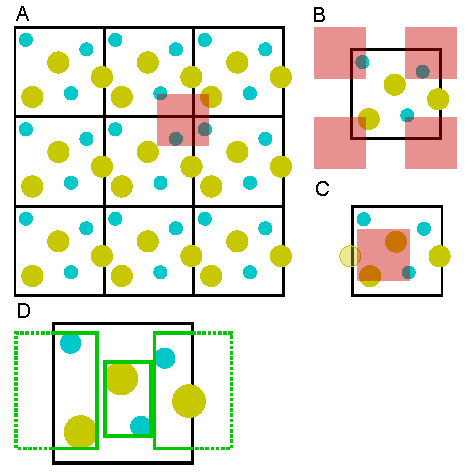
\includegraphics[width=8.4cm, bb=6 3 220 224]{fig1.eps}
    \caption{Methods to handle R-Tree on periodic boundary conditions.
    (\textbf{A})
    By copying the unit cell for each dimension along periodicity, normal R-Tree
    can manage objects that are associated with periodic images.
    (\textbf{B})
    By adding extensional query translated for each periodic images, R-Tree can
    detect objects that are beyond boundary.
    (\textbf{C})
    With the method described in \textbf{B}, finite sized objects could be
    overlooked when queries that is inside of the boundary are not copied.
    (\textbf{D})
    This is the method proposed in this paper. Forming rectangles according to
    the periodicity, R-Tree can organize objects on periodic boundary
    conditions.}
    \label{fig1}
\end{figure}

Here I propose the novel method to apply PBCs to R-Tree. The main idea is
applying the PBCs to each operations for AABBs that are performed in each steps to
maintain an R-Tree. With this method, it is not needed to copy objects or
queries at all. Moreover, using the information about the boundary condition,
it is expected that the size of each AABBs associated with each nodes decreases
relative to the other methods, suggesting that the spatial search become more
efficient.

In section 2, I provide the methods that can be used to grow and maintain the
R-Tree structure. I present the performance results when it is used in the
biochemical simulation in section 3. I make a summary of this paper in section 4.

\section*{Methods}

The operations that are provided in this paper is for handling and modifying
AABBs on PBCs. I do not modify the algorithm to grow and maintain an R-Tree at all.
Hence, in this setion, I do not show algorithm to construct R-Tree itself.
The main algorithm used to make R-Tree in section 3 is completely same as Guttman's
quadratic algorithm.
It means that the operations can potentially be applied for some R-Tree variants
and the other spatial indexing methods that uses AABBs.

Because the rectangles that are used in R-Tree are axis-aligned, it is
enough to show the operation for one dimension to provide the whole algorithm.
Applying those procedure to each dimensions, these operations can easily be
extended for high-dimensional cases.

\paragraph{Representation of the PBCs.}
In this paper, I consider only cuboids as a unit cell of the PBCs.
To describe the boundary conditions, it is enough to show the shape of the unit
cell. As a rectangle, I represent the unit cell as a pair of coordinates showing
upper and lower limit. For efficiency, caching the width of the unit cell in
each dimension might be useful.

To restrict the coordinates to the unit cell, I use the function described in
algorithm\ref{restrict_position}. For the inter coordinate direction, I use the
function shown in algorithm\ref{calc_direction}. 

\begin{algorithm}
    \caption{restrict coordinate to the unit cell of PBCs.}
    \label{restrict_position}
    \begin{algorithmic}
        \State $X  \gets$ coordinate to restrict
        \State $BL \gets$ lower limit of the boundary
        \State $BU \gets$ upper limit of the boundary
        \Function{RestrictPosition}{$X, BL, BU$}
            \State $size \gets BU - BL$
            \If{$X < BL$}
                \State $X \gets X + size$
            \ElsIf{$X \geq BU$}
                \State $X \gets X - size$
            \EndIf
        \EndFunction
     \end{algorithmic}
\end{algorithm}

\begin{algorithm}
    \caption{calculate inter-positional vector on the PBC.}
    \label{calc_direction}
    \begin{algorithmic}
        \State $X1 \gets$ coordinate of starting position
        \State $X2 \gets$ coordinate of stopping position
        \State $BL \gets$ lower limit of the boundary
        \State $BU \gets$ upper limit of the boundary
        \Function{CalcDirection}{$X1, X2, BL, BU$}
            \State $dx \gets X2 - X1$
            \State $size \gets BU - BL$
            \If{$dx > size / 2$}
                \State $dx \gets dx - size$
            \ElsIf{$dx \leq -size / 2$}
                \State $dx \gets dx + size$
            \EndIf
            \State \Return $dx$
        \EndFunction
     \end{algorithmic}
\end{algorithm}

\paragraph{Representation of an AABB.}
There are some options to represent an AABB. To handle AABBs on PBCs efficiently,
here I represent AABBs as pairs of upper and lower limits in each dimensions
(figure \ref{fig2}A).

Restricting positions of both upper and lower limit to inside of the boundary,
the coordinate of upper limit can be lesser than that of lower limit if the AABB
locates over the boundary (figure \ref{fig2}BC). Using this feature, the actual
range occupied by the AABB can be determined easily (algorithm\ref{span}).
If the upper coordinate is same as lower coordinate, it means sizeless box.

\begin{algorithm}
    \caption{calculate the range occupied by the AABB}
    \label{span}
    \begin{algorithmic}
        \State $L  \gets$ lower limit of the box
        \State $U  \gets$ upper limit of the box
        \State $BL \gets$ lower limit of the boundary
        \State $BU \gets$ upper limit of the boundary
        \Function{Span}{$L, U, BL, BU$}
            \If{$U < L$}
                \State $span \gets U - L + (BU - BL)$
            \Else
                \State $span \gets U - L$
            \EndIf
            \State \Return span
        \EndFunction
    \end{algorithmic}
\end{algorithm}

By using the algorithm\ref{span}, the centroid of an AABB can be calculated
easily(algorithm\ref{centroid}).

\begin{algorithm}
    \caption{calculate the centroid of an AABB}
    \label{centroid}
    \begin{algorithmic}
        \State $L  \gets$ lower limit of the box
        \State $U  \gets$ upper limit of the box
        \State $BL \gets$ lower limit of the boundary
        \State $BU \gets$ upper limit of the boundary
        \Function{Centroid}{$L, U, BL, BU$}
            \State $sp \gets$ \Call{Span}{L, U, BL, BU}
            \State $c  \gets$ L + sp / 2
            \State \Return \Call{RestrictPosition}{c, BL, BU}
        \EndFunction
    \end{algorithmic}
\end{algorithm}

To ensure the requirements for AABBs described above, I present a function to
put AABBs inside of the boundary (algorithm\ref{adjust_box}). It checks each
boundary is within the boundary and adjust its position along the conditions.

\begin{algorithm}
    \caption{adjsut upper and lower limit positions of the AABB on PBCs}
    \label{adjust_box}
    \begin{algorithmic}
        \State $L  \gets$ lower limit of the box
        \State $U  \gets$ upper limit of the box
        \State $BL \gets$ lower limit of the boundary
        \State $BU \gets$ upper limit of the boundary
        \Function{RestrictBox}{$L, U, BL, BU$}
            \If{$U - L \geq BU - BL$}
                \State $L \gets BL$
                \State $U \gets BU$
            \ElsIf{$L < BL$}
                \State $L \gets L + (BU - BL)$
            \ElsIf{$BU < U$}
                \State $U \gets U - (BU - BL)$
            \EndIf
            \State \Return
        \EndFunction
     \end{algorithmic}
\end{algorithm}

\paragraph{Expanding AABBs on PBCs.}
Expanding an AABB so that it contains other object completely is one of the most
important operations done to form R-Tree. Because the total area that is covered by
AABBs in the nodes of R-Tree affects the efficiency of spatial searching, it is
needed to find the way to make the expanded area as small as possible.

The algorithm to find minimum expansion of AABB to contain another AABB is shown
in algorithm \ref{expand_aabb_aabb}. The size of bounding box that contains two
rectangles can be calculated as a sum of distance between two centroids of the
rectangles and half-width of the two rectangles (figure \ref{fig-bounding-box}).
Hense, the minimum bounding box on PBCs can be determined by calculating
minimum distance between two centroids of rectangles.

\begin{algorithm}
    \caption{expand AABB so that it contains another AABB}
    \label{expand_aabb_aabb}
    \begin{algorithmic}
        \State $L1 \gets$ lower limit of the box1
        \State $U1 \gets$ upper limit of the box1
        \State $L2 \gets$ lower limit of the box2
        \State $U2 \gets$ upper limit of the box2
        \State $BL \gets$ lower limit of the boundary
        \State $BU \gets$ upper limit of the boundary
        \Function{ExpandAABB}{$L1, U1, L2, U2, BL, BU$}
            \State $s1 \gets$ \Call{Span}{L1, U1, BL, BU}
            \State $s2 \gets$ \Call{Span}{L2, U2, BL, BU}
            \State $c1 \gets$ \Call{Centroid}{L1, U1, BL, BU}
            \State $c2 \gets$ \Call{Centroid}{L2, U2, BL, BU}
            \State $dc \gets$ \Call{CalcDirection}{c1, c2, BL, BU}

            \State $l1 \gets c1 - s1 / 2$
            \State $u1 \gets c1 + s1 / 2$
            \State $l2 \gets c1 + dc - s2 / 2$
            \State $u2 \gets c1 + dc + s2 / 2$

            \State $L1 \gets min(l1, l2)$
            \State $U1 \gets max(u1, u2)$
            \State \Call{RestrictBox}{L1, U1, BL, BU}
            \State \Return
        \EndFunction
     \end{algorithmic}
\end{algorithm}

\paragraph{Checking whether AABB is inside of the other AABB on PBCs.}
Lorem ipsum dolor sit amet, consectetur adipiscing elit. Aliquam bibendum
finibus diam, gravida sagittis lorem gravida vitae. Interdum et malesuada fames
ac ante ipsum primis in faucibus. Nulla in diam tristique ante posuere
tristique. Donec interdum purus sit amet nisl accumsan consectetur. Fusce
aliquet libero mi, quis ornare dolor congue ullamcorper. Nulla nulla urna,
molestie in urna sed, lacinia volutpat eros. Ut mi libero, elementum scelerisque
ipsum vel, hendrerit fermentum turpis. Aliquam sit amet leo sodales, egestas
augue id, fermentum nulla. Aenean vel cursus ante, et pellentesque eros. Nulla
ac neque nec justo posuere commodo sit amet sit amet justo. Aliquam tincidunt
tempor ex nec tincidunt. In ullamcorper vehicula lobortis.

\section*{Results}
\subsection*{subsection 1}
Lorem ipsum dolor sit amet, consectetur adipiscing elit. Aliquam bibendum
finibus diam, gravida sagittis lorem gravida vitae. Interdum et malesuada fames
ac ante ipsum primis in faucibus. Nulla in diam tristique ante posuere
tristique. Donec interdum purus sit amet nisl accumsan consectetur. Fusce
aliquet libero mi, quis ornare dolor congue ullamcorper. Nulla nulla urna,
molestie in urna sed, lacinia volutpat eros. Ut mi libero, elementum scelerisque
ipsum vel, hendrerit fermentum turpis. Aliquam sit amet leo sodales, egestas
augue id, fermentum nulla. Aenean vel cursus ante, et pellentesque eros. Nulla
ac neque nec justo posuere commodo sit amet sit amet justo. Aliquam tincidunt
tempor ex nec tincidunt. In ullamcorper vehicula lobortis.

\subsection*{subsection 2}
Lorem ipsum dolor sit amet, consectetur adipiscing elit. Aliquam bibendum
finibus diam, gravida sagittis lorem gravida vitae. Interdum et malesuada fames
ac ante ipsum primis in faucibus. Nulla in diam tristique ante posuere
tristique. Donec interdum purus sit amet nisl accumsan consectetur. Fusce
aliquet libero mi, quis ornare dolor congue ullamcorper. Nulla nulla urna,
molestie in urna sed, lacinia volutpat eros. Ut mi libero, elementum scelerisque
ipsum vel, hendrerit fermentum turpis. Aliquam sit amet leo sodales, egestas
augue id, fermentum nulla. Aenean vel cursus ante, et pellentesque eros. Nulla
ac neque nec justo posuere commodo sit amet sit amet justo. Aliquam tincidunt
tempor ex nec tincidunt. In ullamcorper vehicula lobortis.

\section*{Discussion}

Lorem ipsum dolor sit amet, consectetur adipiscing elit. Aliquam bibendum
finibus diam, gravida sagittis lorem gravida vitae. Interdum et malesuada fames
ac ante ipsum primis in faucibus. Nulla in diam tristique ante posuere
tristique. Donec interdum purus sit amet nisl accumsan consectetur. Fusce
aliquet libero mi, quis ornare dolor congue ullamcorper. Nulla nulla urna,
molestie in urna sed, lacinia volutpat eros. Ut mi libero, elementum scelerisque
ipsum vel, hendrerit fermentum turpis. Aliquam sit amet leo sodales, egestas
augue id, fermentum nulla. Aenean vel cursus ante, et pellentesque eros. Nulla
ac neque nec justo posuere commodo sit amet sit amet justo. Aliquam tincidunt
tempor ex nec tincidunt. In ullamcorper vehicula lobortis.

\bibliographystyle{plain}
\bibliography{library}{}

\end{document}
